\documentclass[aspectratio=169,10pt]{beamer}

\usetheme{CambridgeUS}
\usecolortheme{dolphin}
\setbeamertemplate{navigation symbols}{}
\setbeamertemplate{footline}[frame number]

\usepackage{amsmath}
\usepackage{amssymb}
\usepackage{booktabs}
\usepackage{graphicx}
\usepackage{tikz}
\usepackage{algorithm}
\usepackage{algorithmic}

\definecolor{darkblue}{RGB}{0,51,102}
\setbeamercolor{structure}{fg=darkblue}

\title{Fixed Income Allocation Strategy}
\author{Taiya Shiva}
\institute{Hawk Center for Investment Analysis\\Regentfund Project}
\date{March 10, 2026}

\begin{document}

\begin{frame}
\titlepage
\end{frame}

\begin{frame}{Outline}
\tableofcontents
\end{frame}

\section{Introduction}

\begin{frame}{Fixed Income Markets and Momentum}
\textbf{Core Premise:} Fixed income markets exhibit time-varying risk premia that can be systematically captured through momentum-based strategies

\vspace{0.4cm}

\textbf{Why momentum works in fixed income:}
\begin{itemize}
    \item Credit spreads widen or tighten gradually as economic conditions evolve, creating persistent price trends

    \item Interest rate regimes exhibit persistence due to central bank policy cycles and slow-moving macroeconomic fundamentals

    \item Rather than exploiting behavioral inefficiencies, momentum signals capture the systematic adjustment of bond prices to fundamental risk factors

    \item Multi-horizon BMOM framework targets these dynamics: 60-120 day lookbacks align to credit cycle frequencies, 240-day lookbacks confirm longer-term interest rate regime shifts
\end{itemize}
\end{frame}

\begin{frame}{Asset Universe and Benchmark}
\textbf{Sample Period:} December 1997 -- November 2025 (27 years, 7,023 daily observations)

\vspace{0.3cm}

\begin{columns}[t]
\column{0.5\textwidth}
\textbf{Three Fixed Income Asset Classes}
\begin{itemize}
    \item \textbf{H5A4 (High Yield)}: ICE BofA US High Yield Index -- non-investment-grade corporate bonds

    \item \textbf{C5A0 (Investment Grade)}: ICE BofA US Investment Grade Corporate Index -- investment-grade corporate debt

    \item \textbf{G5O2 (Government)}: ICE BofA US Treasury Index -- U.S. Treasury bonds as defensive anchor

    \item \textbf{Cash}: 5-10\% buffer depending on market conditions
\end{itemize}

\column{0.5\textwidth}
\textbf{Benchmark Allocation}
\begin{center}
\begin{tabular}{lc}
\toprule
\textbf{Asset} & \textbf{Weight} \\
\midrule
C5A0 (Investment Grade) & 66.5\% \\
H5A4 (High Yield) & 9.5\% \\
G5O2 (Government) & 19.5\% \\
Cash & 5.0\% \\
\bottomrule
\end{tabular}
\end{center}

\vspace{0.2cm}

Regentfund's baseline static allocation that the tactical framework seeks to outperform
\end{columns}
\end{frame}

\begin{frame}{Implementation Constraints}
Two critical constraints shape the final implementation:

\vspace{0.4cm}

\textbf{1. High Yield Cap}
\begin{itemize}
    \item Maximum 12\% allocation to H5A4 (high yield)
    \item Limits credit concentration risk in the Regentfund portfolio
\end{itemize}

\vspace{0.4cm}

\textbf{2. Monthly Rebalancing}
\begin{itemize}
    \item Transaction execution limited to month-end to minimize implementation costs
    \item Exceptions permitted for immediate risk-off signals
\end{itemize}
\end{frame}

\begin{frame}{Strategy Evolution}
This research documents the development process through four stages:

\vspace{0.4cm}

\textbf{Strategy 1: Cross-Asset Momentum Filter}
\begin{itemize}
    \item Establishes binary long/flat signals through cross-asset benchmark filtering and long-term trend confirmation
\end{itemize}

\vspace{0.3cm}

\textbf{Strategy 2: Drawdown Differential Override}
\begin{itemize}
    \item Introduces state machine logic to capitalize on periods when tactical signals successfully avoid losses
\end{itemize}

\vspace{0.3cm}

\textbf{Strategy 3: Proportional Linear Allocation}
\begin{itemize}
    \item Implements portfolio-level allocation across all three assets with constraints
\end{itemize}

\vspace{0.3cm}

\textbf{Monthly Strategy: Operational Implementation}
\begin{itemize}
    \item Optimizes transaction timing through scheduled monthly rebalancing with risk-triggered overrides
\end{itemize}
\end{frame}

\section{Methodology}

\begin{frame}{Signal Generation: Blended Momentum (BMOM)}
\textbf{Foundation:} Multi-horizon momentum indicator combining four distinct lookback periods

\vspace{0.3cm}

$$\text{BMOM}_i(t) = 0.15 \cdot \text{Mom}_{i,20} + 0.35 \cdot \text{Mom}_{i,60} + 0.35 \cdot \text{Mom}_{i,120} + 0.15 \cdot \text{Mom}_{i,240}$$

\vspace{0.3cm}

\textbf{Asymmetric Weighting Rationale:}
\begin{itemize}
    \item \textbf{70\% weight} on 60-120 day lookbacks: align with typical credit cycle frequencies and capture the gradual widening or tightening of credit spreads as economic conditions evolve

    \item \textbf{15\% weight} on 20-day lookback: provides tactical responsiveness to recent price action

    \item \textbf{15\% weight} on 240-day lookback: serves as regime confirmation signal, ensuring alignment with longer-term interest rate trends
\end{itemize}

\vspace{0.2cm}

This weighting structure balances responsiveness with stability, avoiding overreaction to short-term noise while remaining sensitive to persistent credit and duration dynamics
\end{frame}

\begin{frame}{Strategy 1: Cross-Asset Momentum Filter}
\textbf{Key Innovation:} SPY (equity market) as universal benchmark for cross-asset momentum confirmation

\vspace{0.3cm}

\textbf{Signal Logic for Each Asset:}

\vspace{0.2cm}

\textbf{Exit Condition (Signal = 0):} Exit to cash when either cross-below condition is met AND 240-day momentum is negative

$$\text{Exit if: } \left[\text{BMOM}_{\text{asset}} \text{ and } \text{BMOM}_{\text{SPY}} \text{ both cross below } -0.03\right] \land \text{Mom}_{240} < 0$$

\vspace{0.2cm}

\textbf{Entry Condition (Signal = 1):} $\text{BMOM}_{\text{asset}}(t) > 0$

\vspace{0.2cm}

\textbf{Hold:} If neither exit nor entry conditions met, maintain previous signal state
\end{frame}

\begin{frame}{Strategy 1: BMOM Time Series with SPY Filter}
\begin{columns}[c]
\column{0.55\textwidth}
\begin{center}
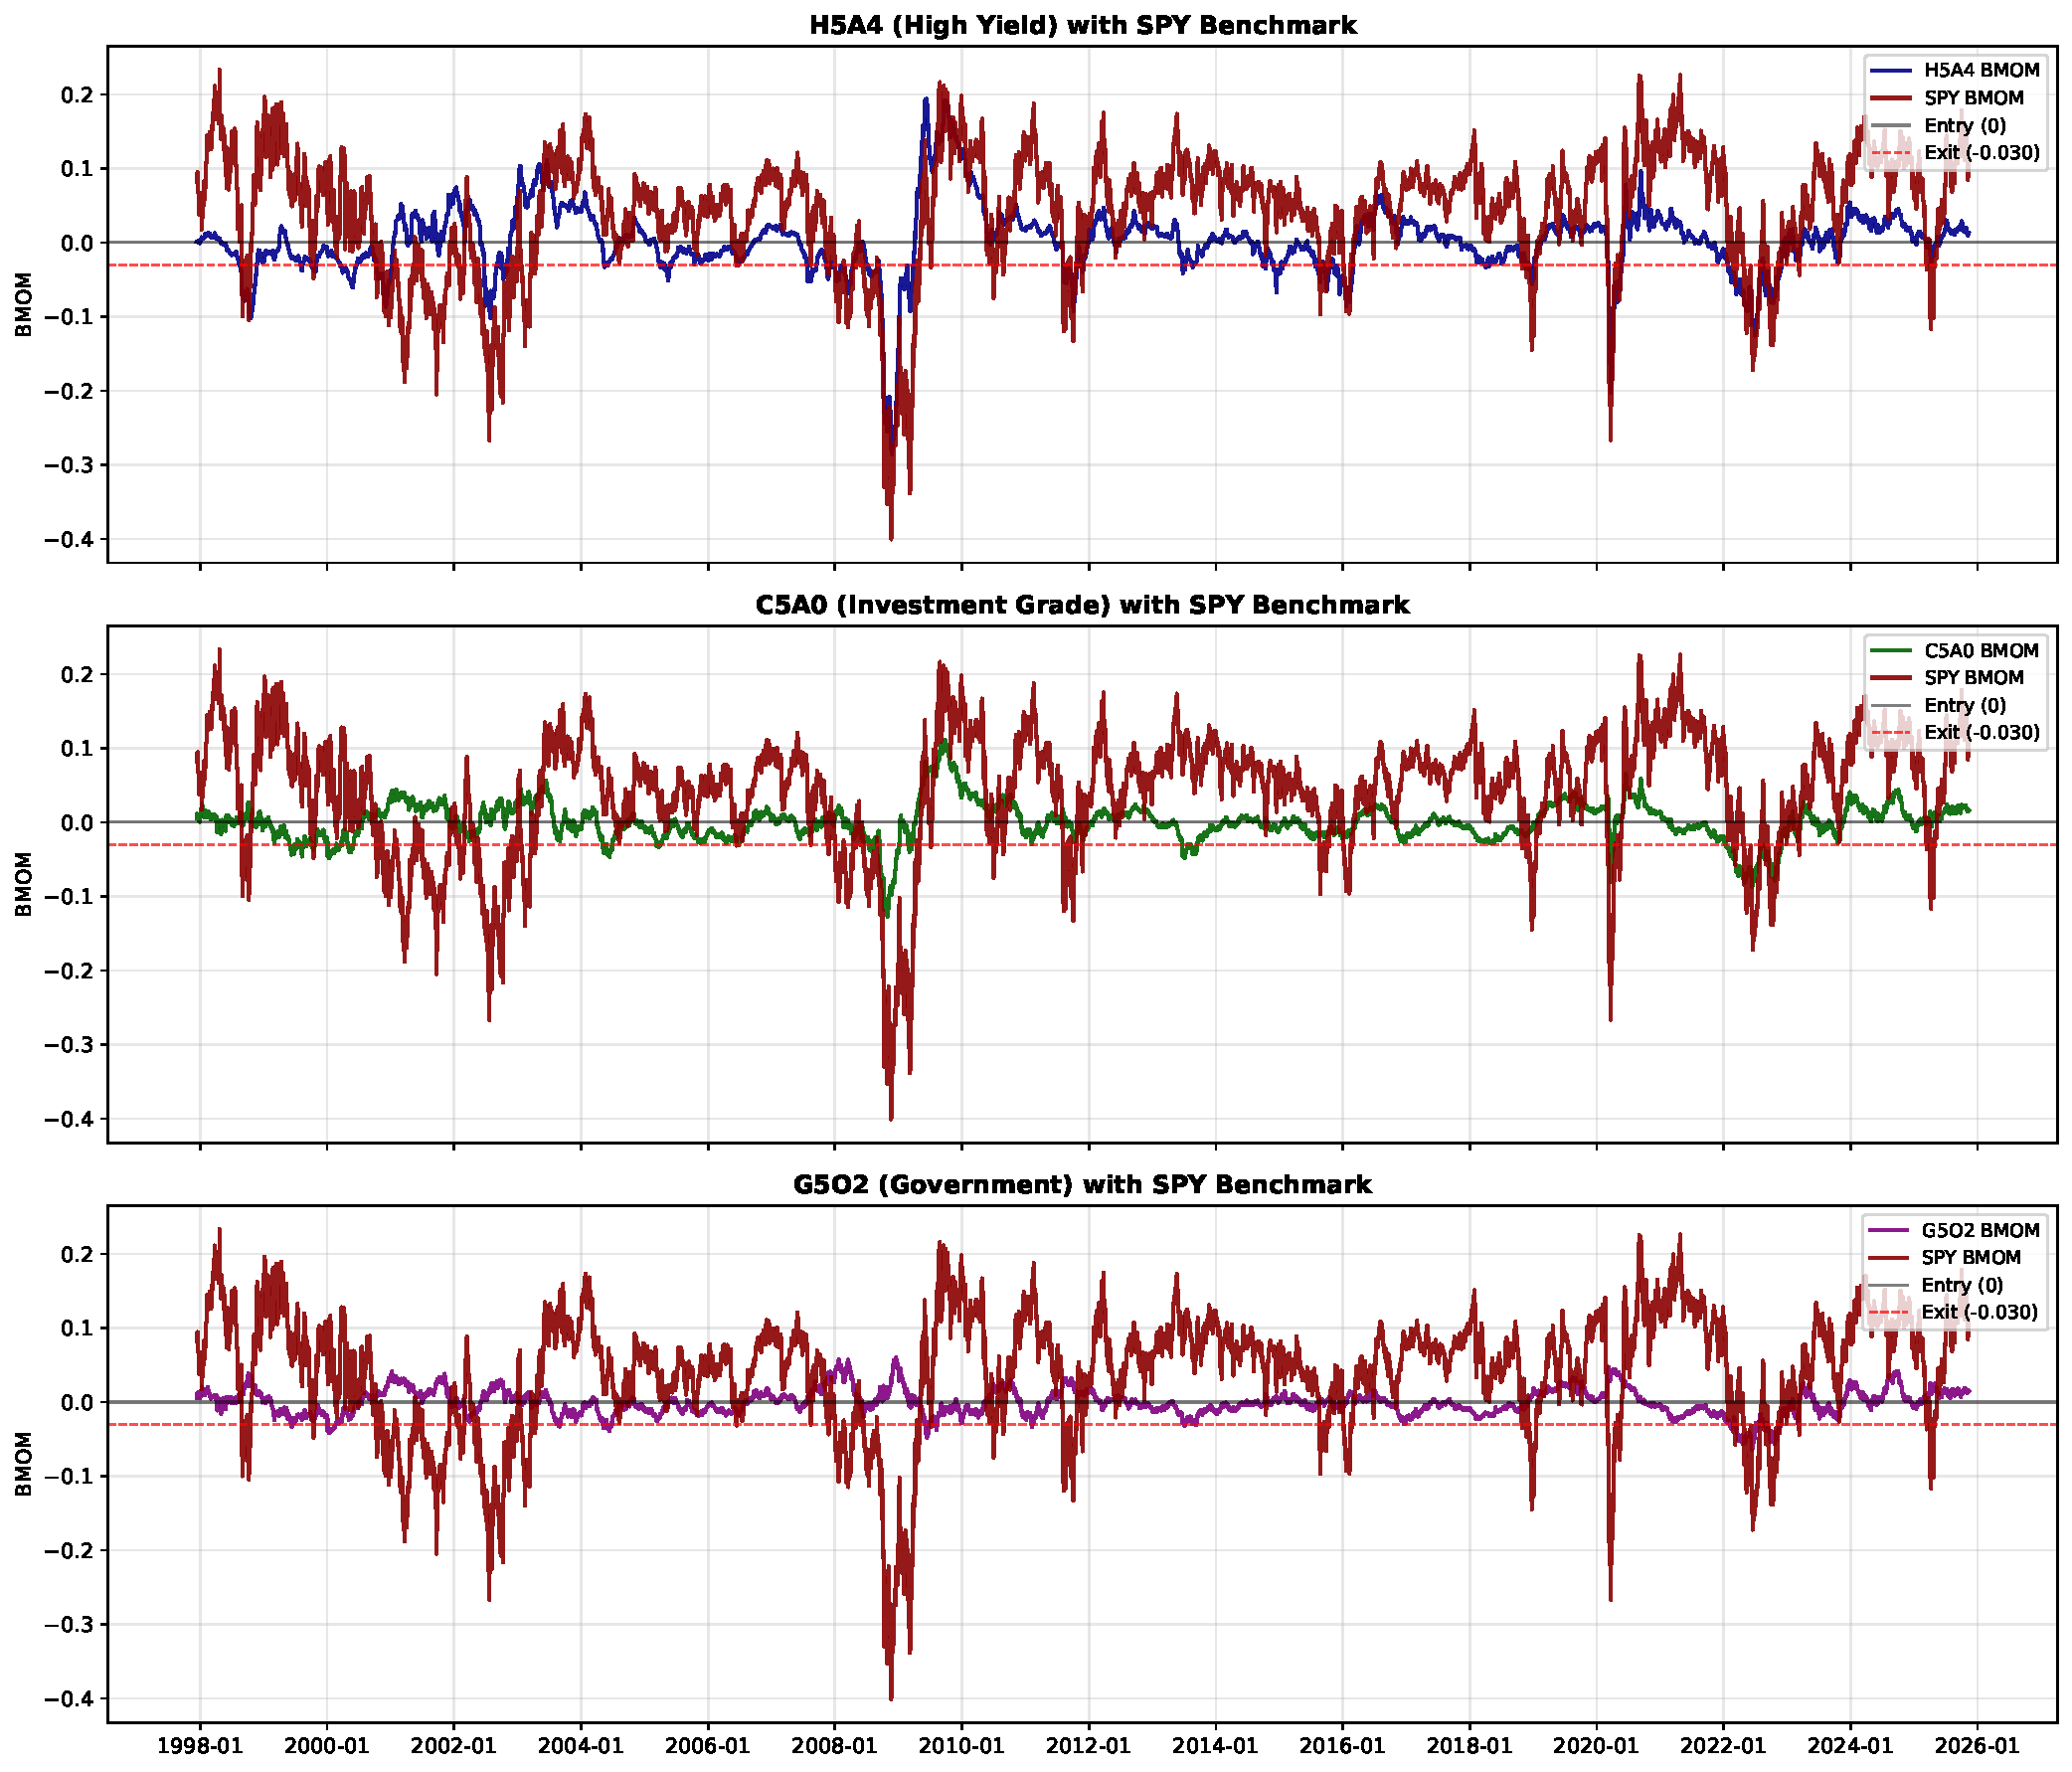
\includegraphics[width=\textwidth]{../PDFs/fig_bmom_timeseries.pdf}
\end{center}

\column{0.42\textwidth}
\textbf{Rationale:}

\vspace{0.2cm}

\small
The largest drawdowns in fixed income assets consistently overlap with periods of SPY BMOM deterioration (2008 financial crisis, 2020 COVID selloff, 2022 interest rate shock).

\vspace{0.2cm}

Dual weakness identifies systemic risk-off periods rather than idiosyncratic volatility.

\vspace{0.2cm}

The cross-asset filter exploits the equity-credit lead-lag relationship: equity markets rapidly incorporate information, while credit markets exhibit delayed price adjustment due to lower liquidity and OTC structure.
\end{columns}
\end{frame}

\begin{frame}{Strategy 1: Asset-Level Results}
\begin{center}
\begin{tabular}{lccc}
\toprule
\textbf{Asset} & \textbf{Ann. Return} & \textbf{Sharpe Ratio} & \textbf{Assessment} \\
\midrule
H5A4 (High Yield) & 0.87\% & 0.24 & Positive \\
C5A0 (Investment Grade) & 0.54\% & 0.18 & Positive \\
G5O2 (Government) & $-0.42\%$ & $-0.14$ & \textcolor{red}{Negative} \\
\bottomrule
\end{tabular}
\end{center}

\vspace{0.4cm}

\textbf{Key Findings:}
\begin{itemize}
    \item Strategy 1's tactical signals successfully avoided losses in credit-sensitive assets (H5A4, C5A0)

    \item Opportunity identified: mechanism needed to remain invested during periods when momentum-based signals prove effective

    \item G5O2 failure reflects difficulty of timing duration exposure through momentum signals
\end{itemize}
\end{frame}

\begin{frame}{Strategy 2: Drawdown Differential Override}
\textbf{Motivation:} Capitalize on periods when tactical signals demonstrably outperform passive exposure

\vspace{0.3cm}

\textbf{Mechanism:} Asset-level drawdown differential override applied independently to each asset

$$\text{DD}_{\text{diff},i}(t) = \text{DD}_{\text{S1},i}(t) - \text{DD}_{\text{BH},i}(t)$$

\vspace{0.2cm}

When $\text{DD}_{\text{diff},i} > 0.10$, Strategy 1's drawdown is more than 10 percentage points less severe than buy-and-hold, indicating the tactical signals are successfully avoiding losses

\vspace{0.3cm}

\textbf{State Machine Architecture:}
\begin{enumerate}
    \item \textbf{Regime Identification:} Each time $\text{DD}_{\text{diff},i}$ crosses above 0.10, a new override regime begins and receives a unique identifier

    \item \textbf{Override Activation:} Signal immediately forced to long (Signal = 1)

    \item \textbf{Regime Persistence:} Long position maintained throughout entire override regime, even if differential subsequently falls below 0.10

    \item \textbf{Strategic Exit:} Override regime only ends when Strategy 1 naturally signals long, ensuring exit occurs when underlying momentum logic confirms continued strength
\end{enumerate}
\end{frame}

\begin{frame}{Strategy 2: Performance Improvement}
\begin{center}
\begin{tabular}{lccc}
\toprule
\textbf{Asset} & \textbf{Strategy 1 Sharpe} & \textbf{Strategy 2 Sharpe} & \textbf{Improvement} \\
\midrule
H5A4 (High Yield) & 0.24 & 0.28 & +16.7\% \\
C5A0 (Investment Grade) & 0.18 & 0.29 & \textbf{+61.1\%} \\
G5O2 (Government) & $-0.14$ & $-0.14$ & 0.0\% \\
\bottomrule
\end{tabular}
\end{center}

\vspace{0.4cm}

\textbf{Critical Findings:}
\begin{itemize}
    \item The substantial improvement in C5A0 demonstrates the override's effectiveness in capturing outperformance during periods when tactical signals successfully navigate credit cycles

    \item No change in G5O2 indicates rare override activation for duration-focused assets

    \item This validates the asset class hypothesis: credit-sensitive assets exhibit exploitable momentum patterns, while Treasury timing remains challenging
\end{itemize}
\end{frame}

\begin{frame}{Proportional Linear Allocation}
\textbf{Objective:} Weight assets by momentum signal strength while enforcing portfolio constraints

\vspace{0.2cm}

\textbf{Allocation Formula:}
$$\text{Score}_i(t) = \max(0, \text{BMOM}_i(t)) \times \text{Signal}_i(t)$$
\vspace{-0.1cm}
$$w_i^{\text{raw}} = \frac{\text{Score}_i}{\sum_j \text{Score}_j} \times 0.95 \quad \text{(5\% cash buffer)}$$

\vspace{0.2cm}

\textbf{Sequential Constraint Enforcement:}
\begin{enumerate}
    \item \textbf{Defensive Mode:} If all scores = 0, allocate 10\% cash and 90\% G5O2
    \item \textbf{Proportional Allocation:} Compute raw weights proportional to scores, normalized to 95\%
    \item \textbf{Minimum Position:} Active assets $<$ 5\% boosted to 5\%, other assets reduced proportionally
    \item \textbf{High Yield Cap:} If H5A4 $>$ 12\%, cap at 12\% and redistribute excess to C5A0, then G5O2, then cash
\end{enumerate}
\end{frame}

\section{Implementation: Monthly Rebalancing Strategy}

\begin{frame}{Monthly Rebalancing Framework}
\textbf{Operational Constraint:} Regentfund Fixed Income Portfolio executes trades on a monthly schedule

\vspace{0.3cm}

\textbf{Dual-Trigger Approach:}

\vspace{0.2cm}

\textbf{1. Scheduled Monthly Rebalancing}
\begin{itemize}
    \item Portfolio weights recalculated and executed on designated monthly trading date
    \item Target weights determined using proportional linear allocation framework with all constraints applied
\end{itemize}

\vspace{0.2cm}

\textbf{2. Risk-Triggered Rebalancing}
\begin{itemize}
    \item When any asset's Strategy 2 signal transitions to 0 (flat), immediately rebalance without waiting for next scheduled date
    \item Weights recalculated with flat asset receiving zero allocation, remaining active assets reweighted proportionally
    \item If all asset signals turn flat simultaneously, shift to defensive mode (10\% cash, 90\% government bonds)
\end{itemize}

\vspace{0.2cm}

Between rebalancing events, portfolio weights drift with market movements
\end{frame}

\section{Results and Performance}

\begin{frame}{Strategy Evolution Performance}
\textbf{Asset-Level Progression (Strategy 1 → Strategy 2):}

\vspace{0.2cm}

\begin{center}
\begin{tabular}{lccc}
\toprule
\textbf{Asset} & \textbf{Strategy 1 Sharpe} & \textbf{Strategy 2 Sharpe} & \textbf{Improvement} \\
\midrule
H5A4 (High Yield) & 0.24 & 0.28 & +16.7\% \\
C5A0 (Investment Grade) & 0.18 & 0.29 & +61.1\% \\
G5O2 (Government) & $-0.14$ & $-0.14$ & 0.0\% \\
\bottomrule
\end{tabular}
\end{center}

\vspace{0.4cm}

\textbf{Portfolio-Level Comparison (Strategy 3 vs. Monthly):}

\vspace{0.2cm}

\begin{center}
\begin{tabular}{lcccc}
\toprule
\textbf{Strategy} & \textbf{Return} & \textbf{Sharpe} & \textbf{Max DD} & \textbf{Trades/Mo} \\
\midrule
Strategy 3 (Daily) & 1.07\% & 0.36 & $-11.71\%$ & 2.79 \\
\textbf{Monthly Strategy} & \textbf{0.77\%} & \textbf{0.26} & \textbf{$-11.99\%$} & \textbf{1.79} \\
\bottomrule
\end{tabular}
\end{center}

\vspace{0.3cm}

The Monthly Strategy represents the implementable version, sacrificing some performance for operational feasibility while maintaining core tactical allocation logic through risk-triggered overrides
\end{frame}

\begin{frame}{Crisis Navigation}
\begin{center}
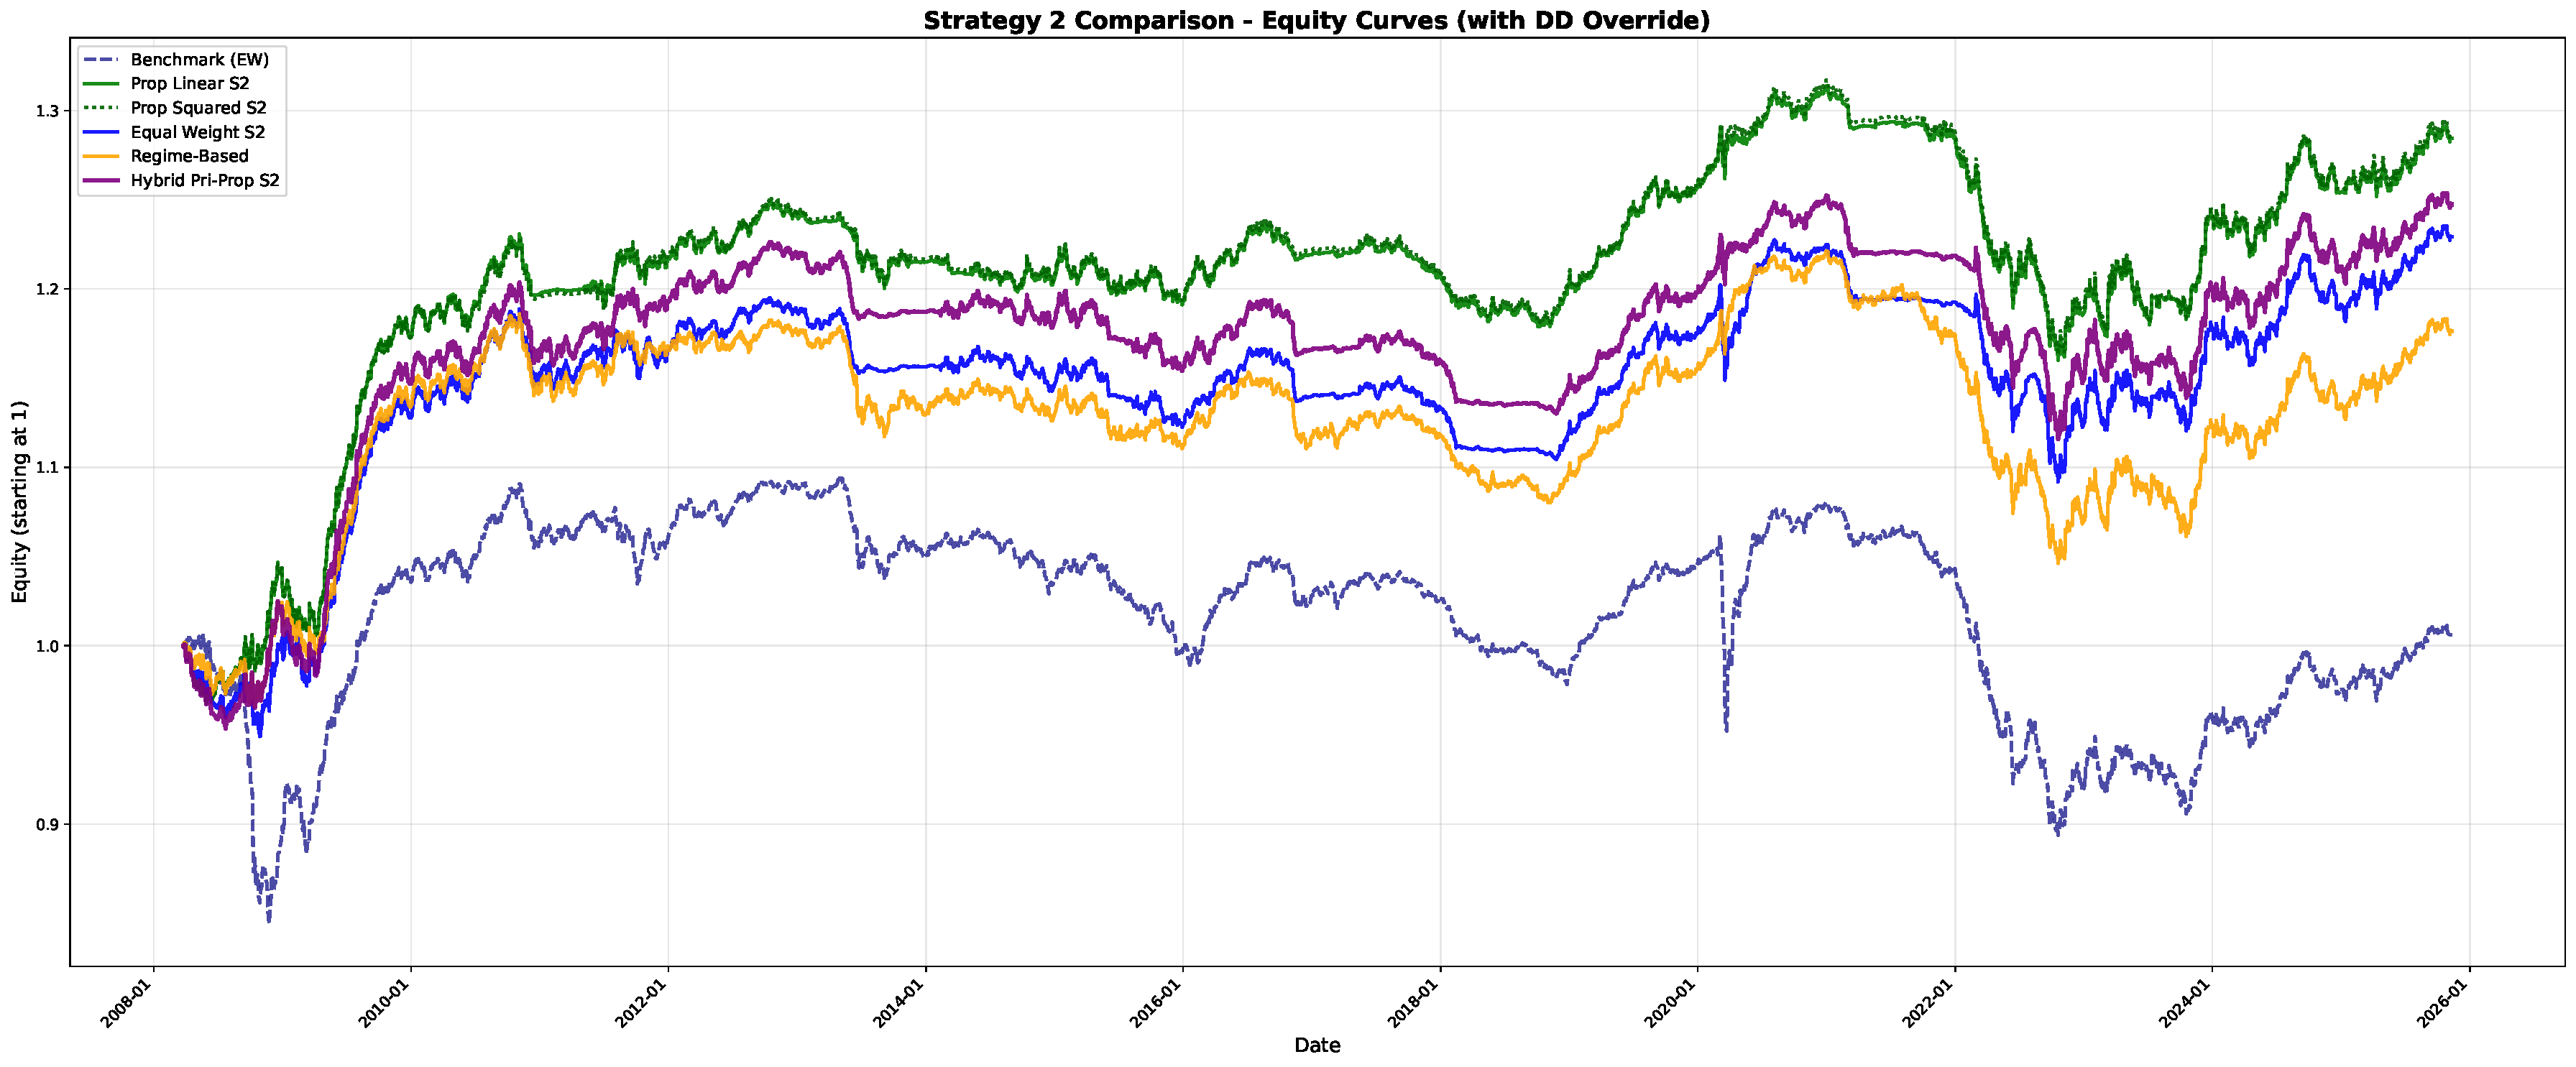
\includegraphics[width=0.75\textwidth]{../PDFs/fig_equity_curves_strat2.pdf}
\end{center}

\vspace{0.2cm}

\small
The framework successfully navigated major market stress events: 2008 financial crisis, 2020 COVID-19 selloff, and 2022 interest rate shock. Both Strategy 3 and Monthly Strategy substantially outperform the static benchmark, with the Monthly Strategy delivering consistent returns while respecting operational trading constraints.
\end{frame}

\section{Conclusion}

\begin{frame}{Conclusion}
\textbf{Deliverable:} Monthly Rebalancing Strategy ready for implementation in Regentfund Fixed Income Portfolio

\vspace{0.4cm}

\textbf{Critical Innovation:} Strategy 2's drawdown differential override was the key breakthrough, particularly for credit-sensitive assets. Rather than simply avoiding losses, the override capitalizes on periods when tactical signals demonstrably outperform passive exposure, forcing positions to remain long until the underlying momentum logic confirms exit timing. This state machine architecture achieved a 61\% Sharpe improvement for C5A0 (investment grade credit).

\vspace{0.4cm}

\textbf{Final Strategy Characteristics:}
\begin{itemize}
    \item 0.26 Sharpe ratio, 0.77\% annualized return, $-11.99\%$ maximum drawdown
    \item 1.79 trades per month (scheduled monthly rebalances + risk-triggered overrides)
    \item Exceeds benchmark by $\geq$10 basis points annualized
    \item Systematic risk management: cross-asset benchmark filtering identifies broad market stress, Mom240 filter prevents exits during temporary pullbacks, dual-trigger rebalancing preserves tactical responsiveness within monthly constraints
\end{itemize}
\end{frame}

\appendix

\section*{Appendix}

\begin{frame}{Appendix: Additional Technical Details}
\textbf{Contents:}

\vspace{0.3cm}

\begin{enumerate}
    \item BMOM Construction Details
    \item Strategy 1 Signal Logic (Pseudocode)
    \item Strategy 2 State Machine Algorithm
    \item Portfolio Construction Constraints
    \item Performance Metrics Definitions
    \item Complete Results Table
\end{enumerate}
\end{frame}

\begin{frame}{Appendix A: BMOM Construction}
\textbf{Implementation Details}

\vspace{0.3cm}

For each asset $i$, compute individual momentum terms:
$$\text{Mom}_{i,n}(t) = \frac{P_i(t) - P_i(t-n)}{P_i(t-n)}$$

\vspace{0.2cm}

Weighted sum:
$$\text{BMOM}_i(t) = \sum_{n \in \{20,60,120,240\}} w_n \cdot \text{Mom}_{i,n}(t)$$

\vspace{0.2cm}

Weights: $w_{20} = 0.15$, $w_{60} = 0.35$, $w_{120} = 0.35$, $w_{240} = 0.15$

\vspace{0.3cm}

\textbf{Data Handling:}
\begin{itemize}
    \item All series aligned to asset index (handles missing SPY dates)
    \item First valid observation at $t = 240$ (longest lookback)
    \item Forward-fill missing values within continuous date ranges
\end{itemize}
\end{frame}

\begin{frame}[fragile]{Appendix B: Strategy 1 Signal Logic}
\small
\begin{algorithmic}[1]
\STATE \textbf{Input:} $\text{BMOM}_{\text{asset}}$, $\text{BMOM}_{\text{SPY}}$, $\text{Mom}_{240}$, threshold $= -0.03$
\STATE \textbf{Initialize:} $\text{Signal}(t=0) = 0$
\FOR{$t = 1$ to $T$}
    \STATE $c_1 \leftarrow (\text{BMOM}_{\text{SPY}}(t-1) > -0.03) \land (\text{BMOM}_{\text{SPY}}(t) < -0.03) \land (\text{BMOM}_{\text{asset}}(t) < -0.03)$
    \STATE $c_2 \leftarrow (\text{BMOM}_{\text{asset}}(t-1) > -0.03) \land (\text{BMOM}_{\text{asset}}(t) < -0.03) \land (\text{BMOM}_{\text{SPY}}(t) < -0.03)$
    \IF{$(c_1 \lor c_2) \land (\text{Mom}_{240}(t) < 0)$}
        \STATE $\text{Signal}(t) \leftarrow 0$ \quad \textit{// Risk-off: exit to cash}
    \ELSIF{$\text{BMOM}_{\text{asset}}(t) > 0$}
        \STATE $\text{Signal}(t) \leftarrow 1$ \quad \textit{// Risk-on: enter long}
    \ELSE
        \STATE $\text{Signal}(t) \leftarrow \text{Signal}(t-1)$ \quad \textit{// Hold previous position}
    \ENDIF
\ENDFOR
\STATE \textbf{Output:} $\text{Signal} \in \{0,1\}^T$
\end{algorithmic}
\end{frame}

\begin{frame}[fragile]{Appendix C: Strategy 2 State Machine}
\small
\begin{algorithmic}[1]
\STATE \textbf{Input:} Strategy 1 signals $s_1(t)$, drawdown differential $\text{DD}_{\text{diff}}(t)$
\STATE \textbf{Initialize:} $\text{regime\_id} = 0$, $s_2(t) = s_1(t)$
\FOR{$t = 1$ to $T$}
    \IF{$\text{DD}_{\text{diff}}(t) > 0.10 \land \text{DD}_{\text{diff}}(t-1) \leq 0.10$}
        \STATE $\text{regime\_id} \leftarrow \text{regime\_id} + 1$ \quad \textit{// New override regime}
    \ENDIF
    \IF{$\text{regime\_id} > 0$}
        \STATE $s_2(t) \leftarrow 1$ \quad \textit{// Override: force long}
        \IF{$s_1(t) = 1$}
            \STATE $\text{regime\_id} \leftarrow 0$ \quad \textit{// Strategic exit: end override}
        \ENDIF
    \ELSE
        \STATE $s_2(t) \leftarrow s_1(t)$ \quad \textit{// Follow Strategy 1}
    \ENDIF
\ENDFOR
\STATE \textbf{Output:} Strategy 2 signals $s_2(t) \in \{0,1\}^T$
\end{algorithmic}
\end{frame}

\begin{frame}{Appendix D: Portfolio Constraints}
\textbf{Sequential Constraint Enforcement}

\vspace{0.3cm}

\textbf{Step 1: Defensive Mode Check}
\begin{itemize}
    \item If $\sum_i \text{Score}_i = 0$ (all signals flat or negative momentum)
    \item Allocate: 10\% Cash, 90\% G5O2
    \item Exit constraint logic
\end{itemize}

\vspace{0.2cm}

\textbf{Step 2: Proportional Weights}
\begin{itemize}
    \item $w_i^{\text{raw}} = \frac{\text{Score}_i}{\sum_j \text{Score}_j} \times 0.95$
    \item 5\% to cash buffer
\end{itemize}

\vspace{0.2cm}

\textbf{Step 3: Minimum Position Enforcement}
\begin{itemize}
    \item For each active asset where $w_i < 0.05$: boost to 5\%
    \item Deficit funded by proportionally reducing other active assets
\end{itemize}

\vspace{0.2cm}

\textbf{Step 4: High Yield Cap}
\begin{itemize}
    \item If $w_{\text{H5A4}} > 0.12$: cap at 12\%
    \item Excess redistributed: first to C5A0, then G5O2, finally cash
\end{itemize}
\end{frame}

\begin{frame}{Appendix E: Performance Metrics}
\textbf{Definitions}

\vspace{0.2cm}

\textbf{Annualized Return:}
$$r_{\text{ann}} = \left(\frac{V_T}{V_0}\right)^{252/T} - 1$$

\vspace{0.1cm}

\textbf{Annualized Volatility:}
$$\sigma_{\text{ann}} = \sigma_{\text{daily}} \times \sqrt{252}$$

\vspace{0.1cm}

\textbf{Sharpe Ratio:} (Assuming zero risk-free rate)
$$\text{SR} = \frac{r_{\text{ann}}}{\sigma_{\text{ann}}}$$

\vspace{0.1cm}

\textbf{Maximum Drawdown:}
$$\text{DD}_{\text{max}} = \max_{t} \left(1 - \frac{V_t}{\max_{s \leq t} V_s}\right)$$

\vspace{0.1cm}

\textbf{Win Rate:}
$$\text{WR} = \frac{\#\{t : r_t > 0\}}{T}$$
\end{frame}

\begin{frame}{Appendix F: Complete Results Table}
\small
\begin{center}
\begin{tabular}{lcccccc}
\toprule
\textbf{Strategy} & \textbf{Return} & \textbf{Vol} & \textbf{Sharpe} & \textbf{Max DD} & \textbf{Win Rate} & \textbf{Trades/Mo} \\
\midrule
\multicolumn{7}{l}{\textit{Strategy 1 (Asset-Level):}} \\
H5A4 & 0.87\% & 3.6\% & 0.24 & -- & -- & -- \\
C5A0 & 0.54\% & 3.0\% & 0.18 & -- & -- & -- \\
G5O2 & $-0.42\%$ & 3.0\% & $-0.14$ & -- & -- & -- \\
\midrule
\multicolumn{7}{l}{\textit{Strategy 2 (Asset-Level):}} \\
H5A4 & 1.20\% & 4.3\% & 0.28 & -- & -- & -- \\
C5A0 & 0.90\% & 3.1\% & 0.29 & -- & -- & -- \\
G5O2 & $-0.42\%$ & 3.0\% & $-0.14$ & -- & -- & -- \\
\midrule
\multicolumn{7}{l}{\textit{Portfolio Strategies:}} \\
Strategy 3 & 1.07\% & 2.95\% & 0.36 & $-11.71\%$ & 50.83\% & 2.79 \\
Monthly & 0.77\% & 2.97\% & 0.26 & $-11.99\%$ & 51.05\% & 1.79 \\
\midrule
\multicolumn{7}{l}{\textit{Benchmark:}} \\
Static & -- & -- & -- & -- & -- & 0.00 \\
\bottomrule
\end{tabular}
\end{center}

\vspace{0.2cm}
\textit{Note: Benchmark = 66.5\% C5A0, 19.5\% G5O2, 9.5\% H5A4, 5\% Cash}
\end{frame}

\end{document}
